\documentclass{article}
\usepackage{nips07submit_e,times}
\usepackage{graphicx}
\usepackage{url}
\bibliographystyle{plain}
%\documentstyle[nips07submit_09,times]{article}

\title{Spatial Relationships in Topic Models}


\author{
Roman Stanchak \\
Department of Computer Science\\
University of Maryland\\
College Park, MD XXXXX \\
\texttt{roman@cs.umd.edu} \\
}

% The \author macro works with any number of authors. There are two commands
% used to separate the names and addresses of multiple authors: \And and \AND.
%
% Using \And between authors leaves it to \LaTeX{} to determine where to break
% the lines. Using \AND forces a linebreak at that point. So, if \LaTeX{}
% puts 3 of 4 authors names on the first line, and the last on the second
% line, try using \AND instead of \And before the third author name.

\begin{document}

%\makeanontitle
\maketitle

\begin{abstract}
	TODO at the end
\end{abstract}

% Introduction, general problem
\section{Introduction}
Traditional topic modeling methods generally assume a 'bag of features' model in which there is no notion of order, location or distance associated with each \textit{feature} in the model.   In the real world, order plays a large role in defining the context in which features can appear.  For instance, the meaning of a textual document is lost if the words are randomly permuted.  Similarly, an image of a human face ceases to be recognizeable if the relative positions of the eyes, nose and mouth are scrambled.  Although topic models have seen much success in their application to various domains, these small example suggest that there is something to be gained by considering the
spatial relationships between features. 

\section{Related Work}
% Background, related work
Spatial relationships have been considered in the context of topic modeling.  Wallach\cite{wallach2006} describes a bigram model for text corpora,  Griffiths and Steyvers \cite{griffiths2005} describe LDA Collocation which also considers bigrams, and Wang extends their results for N-grams \cite{xwang2005}.  These works consider only the sequential order of words, and do not explicitly extend to multi-dimensional spaces.  Topic modeling has been considered in the Computer Vision literature for the problem of general object recognition in images \cite{feifei2004}.  A number of researchers have considered how to integrate spatial relationships with topic models in this context.  Some methods are ad-hoc \cite{lazebnik2006},\cite{russell2006}, while others incorporate spatial location directly into the underlying generative topic model \cite{xwang2007},\cite{sudderth2005}.  The goal of these works is object recognition from images, so evaluation is in terms of recognition rate.  In each work, slightly different features and codebook generation methods are used, and typically only one or two image databases are evaluated.  As a result, it is difficult to assess the relative effectiveness of the addition of spatial information to the topic modeling.
\section{Methods}
\subsection{Algorithms}
\begin{itemize}
	\item Latent Dirichlet Allocation
	\item Author Topic Model
\end{itemize}
\subsection{Inducing a Graph}
\begin{itemize}
	\item K-Nearest Neighbors
	\item Fixed-Radius Neighbors
	\item Delaunay Triangulation
\end{itemize}
\subsection{Evaluation}
% Evaluation to be used
aluated in terms of (a) document modeling and (b) document classification.  Following Hofmann \cite{hofmann99probabilistic}, and Blei \cite{blei02latent}, document modeling will be evaluated in terms of the \textit{perplexity} measure on a held out test set.  Similarly, document classification will be evaluated using standard precision-recall on a held out test set. 

\section{Data}
LabelMe is a web-application that allows casual users to upload photos and then annotate them with tagged polygons \cite{labelme}.  At the time of writing, the full database consists of 162993 images, 43182 of which have at least one annotation.  A subset of the database is available for benchmarking purposes.  The training set contains 2920 images, 32164 total annotations and 127 unique tags.  The test set contains 1033 images and 32853 total annotations.   
\begin{figure}[htb]
	\begin{center}
		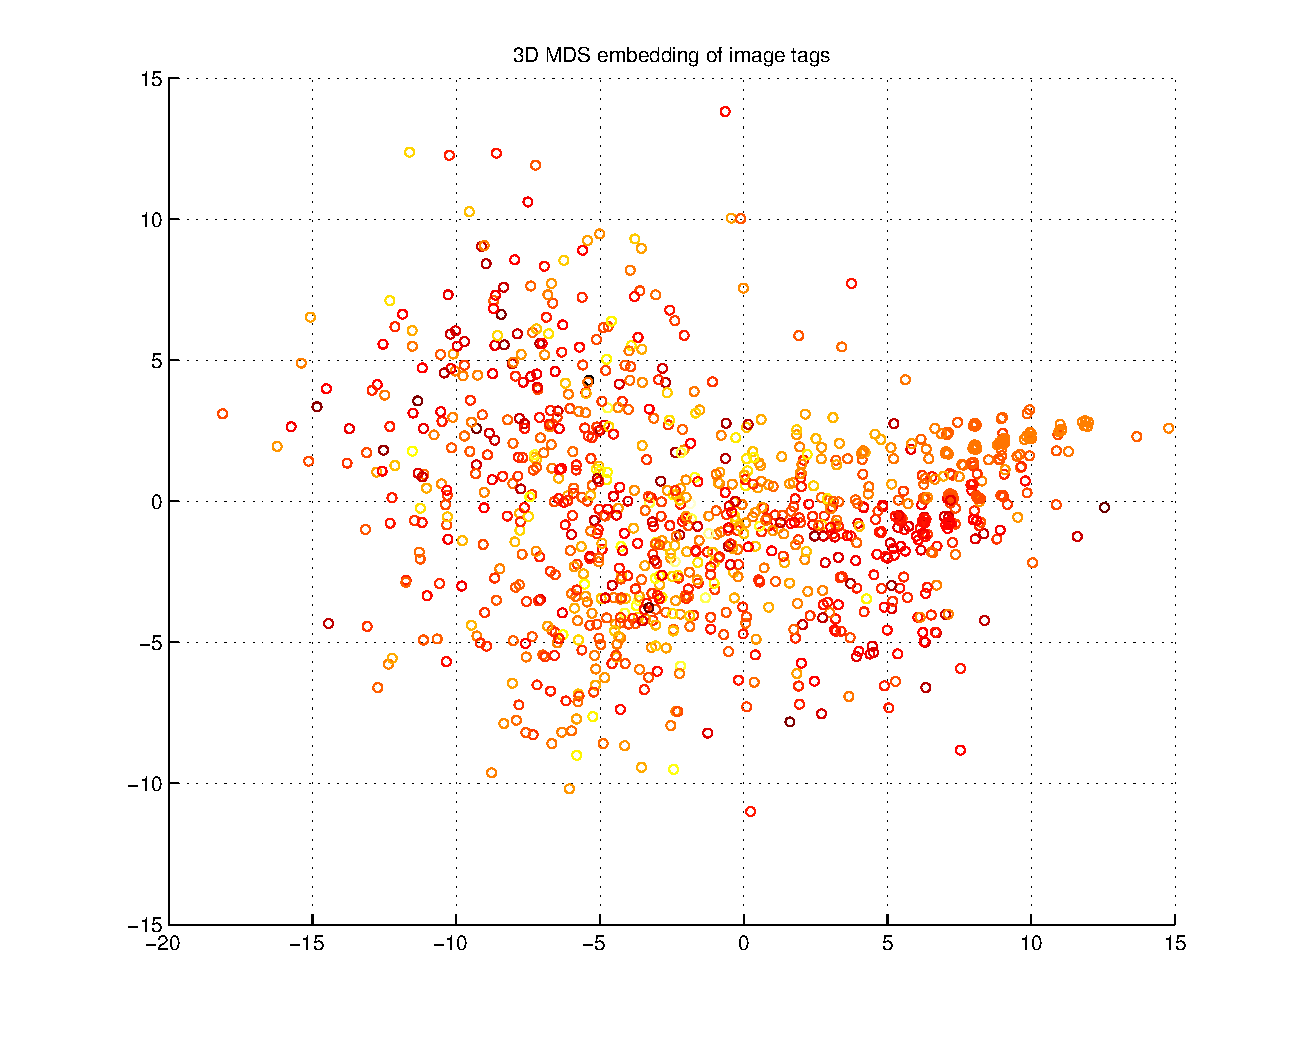
\includegraphics[width=0.5\textwidth]{mds}
	\end{center}
	\caption{MDS embedding of images according to similarity in occurring tags.  The metric used to create the embedding was the L1 distance between the binary tag feature vectors.  }
	\label{fig:MDS}
\end{figure}

\bibliography{stanchak_nips}
\end{document}
